\section{Appendix}

\subsection{Figures for calculation of $E_g$}
\label{sec:appendix_band_gap_plots}
\begin{figure}[htpb]
    \centering
    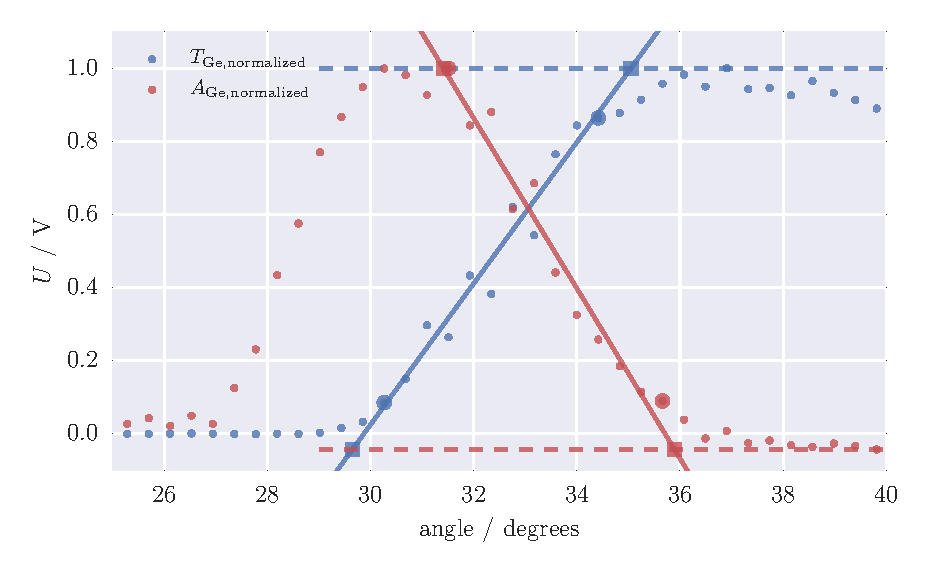
\includegraphics[width=1.0\linewidth]{figures/band_gap_result_Ge_right}
    \caption{
        Result of the procedure fitting straight lines through the points 
        at the transition from transmitting to absorbing characteristic
        for the peaks on the right side ($\alpha > 0$). 
        For indications on the symbols, refer to figure 
        \ref{fig:band_gap_result_Ge_left}. 
        }
    \label{fig:band_gap_result_Ge_right}
\end{figure}

\begin{figure}
    \centering
    \begin{subfigure}[b]{\pltw}
        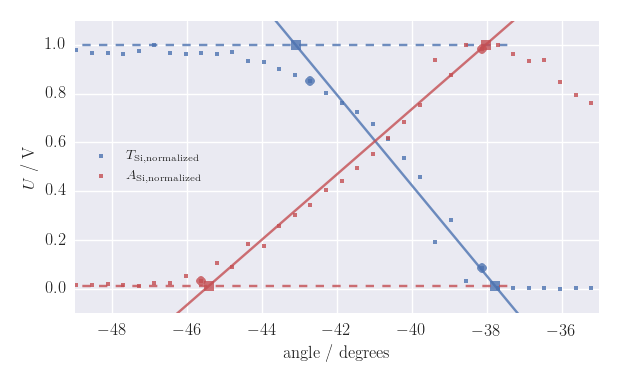
\includegraphics[width=1.0\linewidth]{figures/band_gap_result_Si_left}
        \caption{}
        \label{fig:band_gap_result_Si_left}
    \end{subfigure}
    \begin{subfigure}[b]{\pltw}
        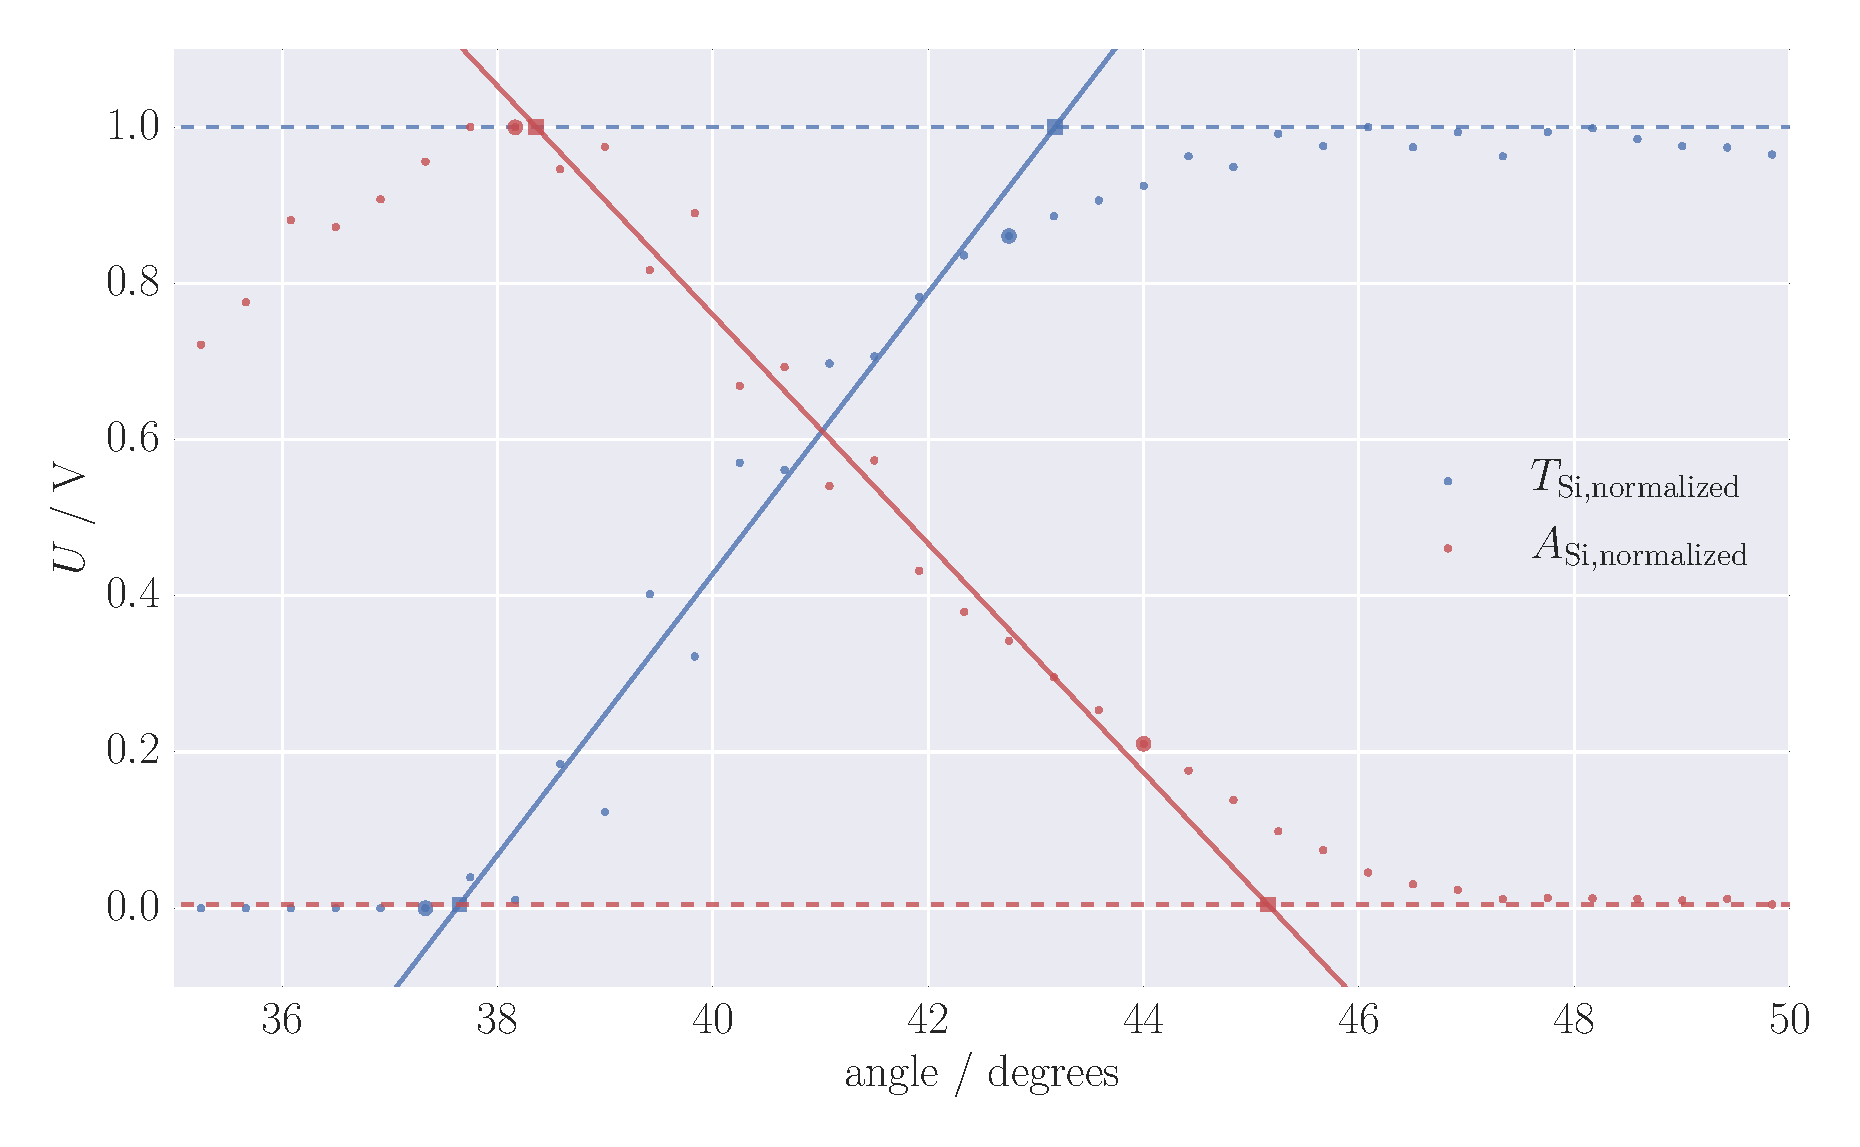
\includegraphics[width=1.0\linewidth]{figures/band_gap_result_Si_right}
        \caption{}
        \label{fig:band_gap_result_Si_right}
    \end{subfigure}
    \caption{
        Result of the procedure fitting straight lines through the points 
        at the transition from transmitting to absorbing characteristic
        for the Si.
        For indications on the symbols, refer to figure 
        \ref{fig:band_gap_result_Ge_left}. 
        }
    \label{fig:band_gap_result_Si}
\end{figure}


\subsection{Appendix: Handwritten records of the experiment}
%    \includegraphics[width=\linewidth]{appendix/}
    \label{sec:records_band_gap}
\clearpage

